\documentclass[twoside,english]{uiofysmaster}

\bibliography{references}


% Adding nicer font to listings
\usepackage{ifxetex}
\ifxetex
  \usepackage{fontspec}
  \newfontfamily\listingsfontfamily[Scale=0.85]{Droid Sans Mono}
  \renewcommand{\listingsfont}{\listingsfontfamily}
\fi


\author{Fredrik Wilhelm Holmen}
\title{Master thesis Wilhelm Coupled Cluster}
\date{Autumn 2015}

\begin{document}
% set space around equations
\setlength{\belowdisplayskip}{12pt} \setlength{\belowdisplayshortskip}{12pt}
\setlength{\abovedisplayskip}{12pt} \setlength{\abovedisplayshortskip}{12pt}


\maketitle

\begin{abstract}
  This is an abstract text.
\end{abstract}

\begin{dedication}
  To someone
  \\\vspace{12pt}
  This is a dedication to my cat.
\end{dedication}

\begin{acknowledgements}
  I acknowledge my acknowledgements.
\end{acknowledgements}

\tableofcontents



\begin{chapter}{Introduction}
  This is a very nice introduction to my myster thesis.
  or ..
  lol
\end{chapter}





\begin{chapter}{Quantum Mechanics}
 	
	

	\begin{section}{Postulates}

 		Quantum 
 	\end{section}

 	\begin{section}{The Born-Oppenheimer Approximation}
 		The Born-Oppenheimer approximation lies at the heart of many-body quantum mechanics. 
 	\end{section}

 	\begin{section}{Pauli's Exclusion Principle}
 		Pauli exclusion principle, also called the antisymmetry principle \cite{Szabo} 
 	\end{section}

	\begin{section}{The Variational Principle}

	\end{section}

	\begin{section}{Slater Determinant}
		A system composed of a nuclei and electrons moving in accordance to the forces of electromagnetic attraction can be described by assigning each electron
		a wave function 
		\begin{align}
			\phi_i(\mathbf{x}_i)
		\end{align}
		Where $\mathbf{x}_i$ is the position vector for the electron i. Describing a system of many electrons can be done writing a Slater Determinant
		\begin{align}
			\ket{\Phi_0} = \frac{1}{ \sqrt{N!} } \left|\begin{matrix}
				\phi_1(\mathbf{x}_1) & \phi_2(\mathbf{x}_1) & ... & \phi_N(\mathbf{x}_1) \\
				\phi_1(\mathbf{x}_2) & \phi_2(\mathbf{x}_2) & ... & \phi_N(\mathbf{x}_2) \\
				... & & & \\
				\phi_1(\mathbf{x}_N) & \phi_2(\mathbf{x}_N) & ... & \phi_N(\mathbf{x}_N) 
			\end{matrix} \right|
		\end{align}
		This way of writing the many-body wave function will represent linear a combination of products of the one-body wave functions $\phi_i$'s and all the electronic coordinates
		$\mathbf{x}_i$ distributed among them in all possible ways. Exchanging two lines will change the sign such that the Slater Determinant will respect the anti-symmetry 
		requirement. \par
		We can choose the one-body wave functions that is most rewarding the specified system. When calculating on electrons moving with respect to a nuclei, one can choose the wave
		functions to be the 1s, 2s, 2p, .. orbitals. This representation will not, however, take into account the Colombic repulsion between two electrons and will only be an 
		approximation to the true wavefunction, $\ket{\Psi}$.
	\end{section}

	\begin{section}{Matrix Elements}
		
	\end{section}

\end{chapter}





\begin{chapter}{Second Quantization}
 	Second quantization is a new method of representing states and operators. 
	\begin{section}{Annihilation and Creation operators}
		We introduce a new way of writing states using the mathematical technique known as second quantization. The main goal is to treat states without paying attention
		to individual particle coordinates. We represent the empty space with the symbol for vacuum
		\begin{align}
			\ket{0}
		\end{align}
		To represent a state, we use a creation operator to add the state to the vacuum.
		\begin{align}
			\hat a_i^{\dagger} \ket{0} = \ket{\phi_i}
		\end{align}
		And the annihilation operator will remove the particle again. 
		\begin{align}
			\hat a_i \ket{\phi_i} = \ket{0}
		\end{align}
		Trying to add a new particle to an already filled state and removing an unoccupied state results in zero.
		\begin{align}
			\hat a_i^{\dagger} \ket{\phi_i} = 0 \;\;\;\;\; \hat a_i \ket{0} = 0
		\end{align}
		Bra states are needed, and by looking at the adjoint of a ket state, we get
		\begin{align}
			\left(\left| \phi_i \right> \right)^\dagger = \left< \phi_i \right| 
		\end{align}
		Which results in
		\begin{align}
			\left( \hat a_i^\dagger \left| 0 \right> \right)^\dagger = \left< 0 \right| \hat a_i = \left< \phi_i \right|
		\end{align}
		We see that the creation and annihilator operatorare each other's adjoint operator. We can define the counting operator, $\hat N$, which will count how many states are occupied in a Slater determinant
		\begin{align}
			\hat N = \sum_p \hat a^\dagger_p \hat a_p = \sum_p \hat n_p
		\end{align}
	\end{section}

	\begin{section}{Strings of Operators}
		We can now construct the Slater determinant by working on vacuum with a string of creation operators
		\begin{align}
			\hat a_1^{\dagger} \hat a_2^{\dagger}... \hat a_N^{\dagger} \ket{0} = \left| \phi_1 \phi_2 ... \phi_N \right>
		\end{align}
		Permutations of the operators introduces a sign-change, which is equivalent to interchanging rows in the determinant. We need second quantization to respect the anisymmetrization condition, so a permutation of two states should introduce a change of sign
		\begin{align}
			\hat a_1^{\dagger} \hat a_2^{\dagger} \ket{0} = \ket{\phi_1 \phi_2} = -\ket{\phi_2 \phi_1} = -\hat a_2^{\dagger} \hat a_1^{\dagger} \ket{0}
		\end{align}
		We introduce the permutation operator, $\hat P$, which permutes two states in the Slater determinant 
		\begin{align}
			\hat P \left| \Phi \right> = (-1)^{\sigma(P)} \left| \Phi \right>
		\end{align}
		Where $\sigma(P)$ counts how many times the states are interchanged. Demonstrated with creation operators
		\begin{align}
			\hat a_1^\dagger \hat a_2^\dagger ... \hat a_i^\dagger \hat a_j^\dagger ... \hat a_n^\dagger = - \hat a_1^\dagger \hat a_2^\dagger ... \hat a_j^\dagger \hat a_i^\dagger ... \hat a_n^\dagger
		\end{align}
	\end{section}

	\begin{section}{Anticommutator Relations}
		When working on strings of operators, it is very convenient to introduce anticommutator relations. We define the relation as 
		\begin{align}
			\{ \hat A, \hat B \} = \hat A \hat B + \hat B \hat A	
		\end{align}
		By inserting the annihilation and creation operator, we can compute the relations and look at how they work on the vacuum state 
		\begin{align}
			\{ \hat a_i^\dagger \hat a_j \} \left| 0 \right>  &= \hat a_i^\dagger \hat a_j \left| 0 \right>  + \hat a_j \hat a_i^\dagger \left| 0 \right> = 0 + \delta_{ij} \left|0\right> 
 		\end{align}
 		Where we have introduced the kroenecker-delta function
 		\begin{align}
 			\delta_{ij} = \begin{cases}
 						1, & \text{if } i = j \\
 						0, & \text{ij } i \neq j
 						\end{cases}
 		\end{align}
		The second case
		\begin{align}
			\{ \hat a_i \hat a_j^\dagger \} \left| 0 \right> &= \hat a_i \hat a_j^\dagger + \hat a_j^\dagger \hat a_i \left| 0 \right> = \delta_{ij} \left| 0 \right> + 0
		\end{align}
		And the two last cases
 		\begin{align}
			\{ \hat a_i \hat a_j \} \left| 0 \right> &= \hat a_i \hat a_j \left| 0 \right> + \hat a_j \hat a_i \left| 0 \right> = \hat a_i \hat a_j \left| 0 \right> - \hat a_i \hat a_j \left| 0 \right> = 0\\
			\{ \hat a_i^\dagger \hat a_j^\dagger \} \left| 0 \right> &= \hat a_i^\dagger \hat a_j^\dagger \left| 0 \right> + \hat a_j^\dagger \hat a_i^\dagger \left| 0 \right> = \hat a_i^\dagger \hat a_j^\dagger \left| 0 \right> - \hat a_i^\dagger \hat a_j^\dagger \left| 0 \right> = 0
 		\end{align}

 		Ending up with our relations
 		\begin{align}
 			&\{ \hat a_i \hat a_j \} = 0 \\
 			&\{ \hat a_i^\dagger \hat a_j^\dagger \} = 0 \\
			&\{ \hat a_i^\dagger \hat a_j \} = \{ \hat a_i \hat a_j^\dagger \} = \delta_{ij}
		\end{align}
		The last result is very useful for rewriting strings of operators, since it allows us to rewrite a set of two operators as
		\begin{align}
			\hat a_i^\dagger \hat a_j = \{ \hat a_i^\dagger \hat a_j \} - \hat a_j \hat a_i^\dagger = \delta_{ij} - \hat a_j \hat a_i^\dagger 
		\end{align}
		Which will be at the center of Wick's theorem. 
	\end{section}

	\begin{section}{Expectation values}
		Doing calculations in many-body quantum mechanics, we are primerely interested in expectation values. It is therefore crucial that we develop a solid scheme for calculating these values. We assume all states are orthonormal, giving
		\begin{align}
			\left< i | j \right> = \delta_{ij}
		\end{align}
		And for consistency, the vacuum state must be normalized
		\begin{align}
			\left< 0 | | 0 \right> = 1
		\end{align}
		because
		\begin{align}
			1 = \left< i | i \right> &= \left< 0 | \hat a_i \hat a_i^\dagger | 0 \right> \\
									 &= \left< 0 | (\{ \hat a_i, \hat a_i^\dagger \} - \hat a_i^\dagger \hat a_i) | 0 \right> \\
									 &= \left< 0 | 0 \right> - 0 = \left< 0 | 0 \right>
		\end{align}



	\end{section}

	

	\begin{section}{Representation of Operators}
		Consider a symmetric one-body operator represented by
		\begin{align}
			\hat F = \sum_{\mu = 1}^N \hat f_\mu 
		\end{align}
		The number $\mu$ tells us on which particle $\hat F$ works on. In this case, we are looking at a symmetric operator because it works identically on all particles. Looking at a matrix element of $\hat F$ put petween two Slater determinants. 
		\begin{align}
			\left< a_1 a_2 ... a_N \right| \hat F \left| b_1 b_2 ... b_N \right> 
		\end{align}
		\begin{align}
			\sum_\mu \left< a_1 a_2 ... a_N \right| \hat f_\mu \left| b_1 b_2 ... b_N \right> 
		\end{align}
	\end{section}

 \begin{section}{Fermi Vacuum}
 	
 \end{section}

 \begin{section}{Normal Ordering and Wick's Theorem}
 	
 \end{section}

 \begin{section}{Partitioning the Hamiltonian}
 	
 \end{section}
 
\end{chapter}




\begin{chapter}{Many-Body Methods}
	We have already justified the use of a Slater Determinant to describe the first approximation of the full wave function, $\ket{\Psi}$. Where
	\begin{align}
		\ket{\Psi} \approx \ket{\Phi_0} = 	\frac{1}{ \sqrt{N!} } \left|\begin{matrix}
			\phi_1(\mathbf{x}_1) & \phi_2(\mathbf{x}_1) & ... & \phi_N(\mathbf{x}_1) \\
			\phi_1(\mathbf{x}_2) & \phi_2(\mathbf{x}_2) & ... & \phi_N(\mathbf{x}_2) \\
			... & & & \\
			\phi_1(\mathbf{x}_N) & \phi_2(\mathbf{x}_N) & ... & \phi_N(\mathbf{x}_N) 
		\end{matrix} \right|
	\end{align}	
	This first representation fails to account for the Coulombic interrraction between the electrons, and we need higher-order approximations on top 
	of the Slater Determinant to improve our results. \par
	This chapter will look at three methods, namely the Configuration interraction, Many-body Perturbation theory and Hartree-Fock approximations. The
	Master thesis is on Coupled Cluster theory, and that will be more elaborately explained in it's own chapter. It is useful to benchmark Coupled Cluster 
	with similar many-body method. 

 \begin{section}{Configuration Interraction}
 		We can write the configuration interaction wavefunction as 
  	\begin{align}
  		\ket{\Psi_{CI}} = (1 + \hat C) \ket{\Phi_0} 
   	\end{align}
  	\begin{align}
  		\hat C = \hat C_1 + \hat C_2 + ... =  \sum_{ia} c_i^a a_a^{\dagger} a_i + \frac{1}{4} \sum_{ijab} c_{ij}^{ab} a_a^{\dagger} a_b^{\dagger} a_j a_i + ...
   	\end{align}
 \end{section}	

 \begin{section}{Many-body Perturbation Theory}
 	
 \end{section}

 \begin{section}{Hartree-Fock approximations}
 	
 \end{section}

\end{chapter}




\begin{chapter}{Coupled-Cluster Theory}
 	In Coupled Cluster theory, the ansatz we make is to make an expansion in the wave function
 	\begin{align}
 		\ket{\Psi} \approx e^{\hat T} \ket{\Psi_0}
  	\end{align}
  	The operator $\hat T$ is a linear combination of the cluster operators
  	\begin{align}
  		\hat T = \hat T_1 + \hat T_2 + \hat T_3 + ... + \hat T_N
  	\end{align}
  	Where the operators represent
  	\begin{align}
  		T_1 &= \sum_{ia} t_i^a \hat a_a^{\dagger} \hat a_i \\
  		T_2 &= \frac{1}{2} \sum_{ijab} t_{ij}^{ab} \hat a_a^{\dagger}\hat a_b^{\dagger} \hat a_j \hat a_i \\
  		T_2 &= \left(\frac{1}{n!}\right)^2 \sum_{ij..ab..}^n t_{ij..n}^{ab..n} \hat a_a^{\dagger}\hat a_b^{\dagger} ...\hat a_n^{\dagger} \hat a_n ... \hat a_j \hat a_i \\
  	\end{align}

  	We can write the configuration interaction wavefunction as 
  	\begin{align}
  		\ket{\Psi_{CI}} = (1 + \hat C) \ket{\Phi_0} 
   	\end{align}
  	\begin{align}
  		\hat C = \hat C_1 + \hat C_2 + ... =  \sum_{ia} c_i^a a_a^{\dagger} a_i + \frac{1}{4} \sum_{ijab} c_{ij}^{ab} a_a^{\dagger} a_b^{\dagger} a_j a_i + ...
   	\end{align}
   	Comparing this linear expansion to the exponential expansion from Coupled Cluster, we can see that
   	\begin{align}
   		\hat C_2 = \hat T_2 + \frac{1}{2} T_1^2
   	\end{align}
   	Where we can see that even if we truncate Configuration Interaction and Coupled Cluster at the same level, there are more \textit{disconnected} wave function contributions (REFERENCE page 17 IN C\&S) in the Coupled Cluster theory. Both the Coupled Cluster and Configuration Interaction theory provides the exact energy by including the operators to infinite order, i.e. no truncation. 

  	\begin{section}{Size Extensivity}
  		It can be important to have a wave function that scales with size. Imagine a two particles, $X$ and $Y$ with infinity separation, they do not interact. This means we should be able to write the total energy as
  		\begin{align}
  			E = E_X + E_Y
  		\end{align}
  		Doing Coupled Cluster
  		\begin{align}
  			\hat T = \hat T_X + \hat T_Y 
  		\end{align}
  		\begin{align}
  			\ket{\Psi}_{CC} = e^{\hat T_X + \hat T_Y} \ket{\Phi_0} = e^{\hat T_X} e^{\hat T_Y} \ket{\Psi_0}
  		\end{align}
  		Since we can write the reference state as a product of the two seperated parts, we are able to write
  		\begin{align}
  			E_{CC} = E_{CC}^X + E_{CC}^Y
  		\end{align}
  		This means Coupled Cluster is size extensive, contrary to the Configuration Interaction. 
  	\end{section}

  	\begin{section}{The CCD Equations}
  		The Coupled Cluster Doubles equations can be finalized as
  		\begin{align}
  			E_{CCD} = E_{ref} + \Delta E_{CCD} 
  		\end{align}
  		With the reference energy defined as 
  		\begin{align}
  			E_{ref} = \sum_i \left< i \middle| \hat h_0 \middle| j\right> + \sum_{ij} \left<ij\middle|\hat v\middle|ij\right> + \frac{1}{2}Av_0
  		\end{align}
  		and the corrolation energy given by
  		\begin{align}
  			\Delta E_{CCD} = \frac{1}{4} \sum_{ijab}\left<ij\middle|\hat v\middle|ab\right> t_{ij}^{ab}
  		\end{align}
  		$v_0$ is a constant, nonzero for the finite electron gas. After several applications of Wick's theorem, the amplitude equations can be reduced to
  		\begin{align}
  			(\epsilon_i + \epsilon_j - \epsilon_a - \epsilon_b) t_{ij}^{ab} = \left<ab\middle|\hat v\middle|ij\right> + \frac{1}{2} \sum_{cd}\left<ab\middle|\hat v\middle|cd\right>t_{ij}^{cd} \\
  			+ \frac{1}{2} \sum_{kl} \left<kl\middle|\hat v\middle|ij\right>t_{kl}^{ab} + \hat P\left(ij\middle|ab\right) \sum_{kc}\left<kb\middle|\hat v\middle|cj\right>t_{ik}^{ac} \\
  			+ \frac{1}{4} \sum_{klcd}\left<kl\middle|\hat v\middle|cd\right>t_{ij}^{cd} t_{kl}^{ab} + \frac{1}{2} \hat P\left(ij\middle|ab\right) \sum_{klcd}\left<kl\middle|\hat v\middle|cd\right>t_{ik}^{ac} t_{lj}^{db}\\
  			- \frac{1}{2}\hat P(ij) \sum_{klcd}\left<kl\middle|\hat v\middle|cd\right>t_{ik}^{ab} t_{jl}^{cd} - \frac{1}{2}\hat P(ab) \sum_{klcd}\left<kl\middle|\hat v\middle|cd\right>t_{kl}^{bd} t_{ij}^{ac}
  			\label{CCD_equations1}
  		\end{align}
  		Where we have defined
  		\begin{align}
  			\hat P(ij) = 1 - \hat P_{ij}
  		\end{align}
  		Where $\hat P_{ij}$ interchanges the two particles occupying the quantum states $i$ and $j$. Furthermore, we define the operator 
  		\begin{align}
  			\hat P\left( ij \middle| ab \right) = (1 - \hat P_{ij}) (1 - \hat P_{ab})
  		\end{align}
  		We notice that some parts are linear in the amplitude, while some are quadradic. Sorting them into the linear and quadradic parts, $L$ and $Q$ respectably, I get
  		\begin{align}
  			L(t_{ij}^{ab}) = \frac{1}{2} \sum_{cd}\left<ab\middle|\hat v\middle|cd\right>t_{ij}^{cd} + \frac{1}{2} \sum_{kl} \left<kl\middle|\hat v\middle|ij\right>t_{kl}^{ab} + \hat P\left(ij\middle|ab\right) \sum_{kc}\left<kb\middle|\hat v\middle|cj\right>t_{ik}^{ac}
  		\end{align}
  		and 
  		\begin{align}
  			Q(t_{ij}^{ab}t_{ij}^{ab}) = \frac{1}{4} \sum_{klcd}\left<kl\middle|\hat v\middle|cd\right>t_{ij}^{cd} t_{kl}^{ab} + \frac{1}{2} \hat P\left(ij\middle|ab\right) \sum_{klcd}\left<kl\middle|\hat v\middle|cd\right>t_{ik}^{ac} t_{lj}^{db} \\
  			- \frac{1}{2}\hat P(ij) \sum_{klcd}\left<kl\middle|\hat v\middle|cd\right>t_{ik}^{ab} t_{jl}^{cd} - \frac{1}{2}\hat P(ab) \sum_{klcd}\left<kl\middle|\hat v\middle|cd\right>t_{kl}^{bd} t_{ij}^{ac}
  		\end{align}
  		Labeling each term for practical reasons	
  		\begin{align}
  			L_a &= \frac{1}{2} \sum_{cd}\left<ab\middle|\hat v\middle|cd\right>t_{ij}^{cd} \\
  			L_b &= \frac{1}{2} \sum_{kl} \left<kl\middle|\hat v\middle|ij\right>t_{kl}^{ab} \\
  			L_c &= \hat P\left(ij\middle|ab\right) \sum_{kc}\left<kb\middle|\hat v\middle|cj\right>t_{ik}^{ac} \\
  			Q_a &= \frac{1}{4} \sum_{klcd}\left<kl\middle|\hat v\middle|cd\right>t_{ij}^{cd} t_{kl}^{ab} \\
  			Q_b &= \frac{1}{2} \hat P\left(ij\middle|ab\right) \sum_{klcd}\left<kl\middle|\hat v\middle|cd\right>t_{ik}^{ac} t_{lj}^{db} \\
  			Q_c &= - \frac{1}{2}\hat P(ij) \sum_{klcd}\left<kl\middle|\hat v\middle|cd\right>t_{ik}^{ab} t_{jl}^{cd} \\
  			Q_d &= - \frac{1}{2}\hat P(ab) \sum_{klcd}\left<kl\middle|\hat v\middle|cd\right>t_{kl}^{bd} t_{ij}^{ac}
  		\end{align}
   	\end{section}

  	\begin{section}{Intermediates}
  		As Coupled Cluster computations are consume large amounts of computational power, researchers are spending much effort trying to reduce computational cost. One way of reducing the cost is by refactoring the amplitude equations such that we can perform an intermediate computation first and use the result to compute various diagrams later. 

  		Rewriting the equation, (\ref{CCD_equations1}) for CCD amplitudes (Source: Gustav Baardsen / Audun):
  		\begin{align}
  			(\epsilon_i + \epsilon_j - \epsilon_a - \epsilon_b) t_{ij}^{ab} = \left<ab\middle|\hat v\middle|ij\right> + \frac{1}{2} \sum_{cd}\left<ab\middle|\hat v\middle|cd\right>t_{ij}^{cd} \\
  			+ \frac{1}{2} \sum_{kl} t_{kl}^{ab} \left[ \left<kl\middle|\hat v\middle|ij\right> + \frac{1}{2} \sum_{cd} \left<kl\middle|\hat v\middle|cd\right> t_{ij}^{cd} \right] \\
  			+ \hat P\left(ij\middle|ab\right) \sum_{kc} t_{ik}^{ac} \left[ \left<kb\middle|\hat v\middle|cj\right> + \frac{1}{2}\sum_{ld}\left<kl\middle|\hat v\middle|cd\right>t_{lj}^{db} \right] \\
  			- \frac{1}{2} \hat P(ij) \sum_{k} t_{ik}^{ab} \left[ \sum_{lcd} \left<kl\middle|\hat v\middle|cd\right> t_{jl}^{cd} \right] \\
  			- \frac{1}{2} \hat P(ab) \sum_{c} t_{ij}^{ac} \left[ \sum_{kld} \left<kl\middle|\hat v\middle|cd\right> t_{kl}^{bd} \right]
  		\end{align}
  		We can now define, and precompute the following values
  		\begin{align}
  			I_1 = \left<kl\middle|\hat v\middle|ij\right> + \frac{1}{2} \sum_{cd} \left<kl\middle|\hat v\middle|cd\right> t_{ij}^{cd} \\
  			I_2 = \left<kb\middle|\hat v\middle|cj\right> + \frac{1}{2}\sum_{ld}\left<kl\middle|\hat v\middle|cd\right>t_{lj}^{db} \\
  			I_3 = \sum_{lcd} \left<kl\middle|\hat v\middle|cd\right> t_{jl}^{cd} \\
  			I_4 = \sum_{kld} \left<kl\middle|\hat v\middle|cd\right> t_{kl}^{bd}
  		\end{align}
  		We can now redefine the CCD equation 
  		\begin{align}
  			(\epsilon_i + \epsilon_j - \epsilon_a - \epsilon_b) t_{ij}^{ab} = \left<ab\middle|\hat v\middle|ij\right> + \frac{1}{2} \sum_{cd}\left<ab\middle|\hat v\middle|cd\right>t_{ij}^{cd} + \frac{1}{2} \sum_{kl} t_{kl}^{ab} I_1 \\
  			+ \hat P\left(ij\middle|ab\right) \sum_{kc} t_{ik}^{ac} I_2 - \frac{1}{2} \hat P(ij) \sum_{k} t_{ik}^{ab} I_3  - \frac{1}{2} \hat P(ab) \sum_{c} t_{ij}^{ac} I_4
  			\label{Intermediates}
  		\end{align}
  		Leading to a reduction of computational cost from $\mathcal{O}(h^4 p^4)$ to $\mathcal{O}(h^4 p^2)$


  	\end{section}

\end{chapter}




\begin{chapter}{The Pairing Model}
	The first system I look at is the pairing model. The pairing model has four energy levels with degeneracy two, one for positive and negative spins. I have 
	used a system consisting of four electrons filling up the four lower-most states up to the Fermi level. 
	\begin{figure}[h]
		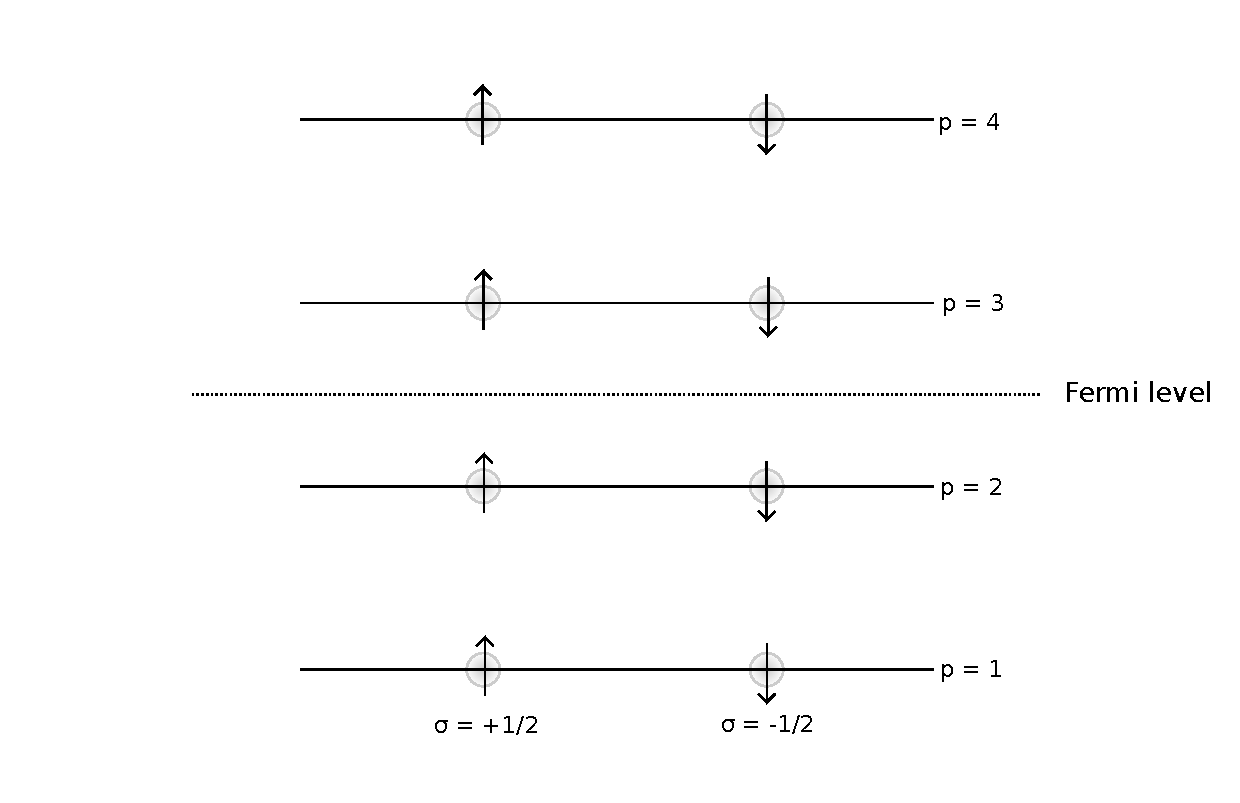
\includegraphics[width=\textwidth]{Figures/Pairing_model.pdf}
		\label{PairingModel_1}
		\caption{A figure depicting a 4 particles-4 holes state. The system consists of occupied particle states below the Fermi level and unoccupied hole states above Fermi level.}
	\end{figure}
	
	\begin{section}{The Hamiltonian}
		We limit ourselves to a two-body interaction, writing the Hamiltonian as
		\begin{align}
			\hat H = \sum_{\alpha \beta} \left< \alpha \right| \hat h_0 \left| \beta \right> \hat a_{\alpha}^{\dagger} \hat a_{\beta} 
			        + \frac{1}{4} \sum_{\alpha \beta \gamma \delta} \left< \alpha \beta \middle| \hat v_0 \middle| \gamma \delta \right> \hat a_{\alpha}^{\dagger} \hat a_{\beta}^{\dagger} \hat a_{\delta} \hat a_{\gamma}
		\end{align}
		We use the complete basis $\left| \alpha \right>$ and define the set as eigenvalues of the one-body operator, $\hat h_0$. 
		
		The system does require that the total spin is equal to $0$. In addition we will not allow spin pairs to be broken, i.e.\  singly excitated states are not allowed. 
		\begin{align}
			\left| \Psi_i^a \right> = 0 
		\end{align}	
		We introduce the double creation and annihilation operator. 
		\begin{align}
			\hat P_{pq}^{\dagger} = \hat a_{p \sigma}^{\dagger} \hat a_{p -\sigma}^{\dagger}
		\end{align}
		\begin{align}
			\hat P_{pq} =  a_{q \sigma} a_{q -\sigma}
		\end{align}

		We can rewrite the Hamiltonian as an unperterturbed part and a perturbation
		\begin{align}
			\hat H = \hat H_0 + \hat V
		\end{align}
		\begin{align}
			\hat H_0 = \xi \sum_{p \sigma} (p-1) \hat a_{p \sigma}^{\dagger} \hat a_{p \sigma}
		\end{align}
		\begin{align}
			\hat V = - \frac{1}{2}g \sum_{pq} \hat a_{p +}^{\dagger} \hat a_{p-}^{\dagger} \hat a_{q-} \hat a_{q+}
		\end{align}
		The value of $\xi$ determines the spacing between the energy levels, which I have set to $1$. This will not impact the insight attained solving this system. $p$ and $q$ determines the energy level. $\sigma$ is the spin, with value either $+\frac{1}{2}$ or $-\frac{1}{2}$. Both the unperturbed and perturbed Hamiltonian keeps total spin at $0$

		We can normal order the Hamiltonian by Wicks general theorem. 
		\begin{align}
			a_p^{\dagger} a_q = \left\{ a_p^{\dagger}a_q \right\} + \delta_{pq \in i}
		\end{align}
		\begin{align}
			a_p^{\dagger} a_q^{\dagger} a_s a_r = \left\{ a_p^{\dagger}a_q^{\dagger} a_s a_r \right\} +\left\{a_p^{\dagger}a_r\right\} \delta_{qs\in i} - \left\{a_p^{\dagger}a_s\right\} \delta_{qr\in i} \\
			+\left\{a_q^{\dagger}a_s\right\} \delta_{pr\in i} \
			- \left\{a_q^{\dagger}a_r\right\} \delta_{ps\in i} + \delta_{pr \in i} \delta_{qs \in i} - \delta_{ps \in i}\delta_{qr \in i}
		\end{align}
		Which gives the Normal-ordered Hamiltonian
		\begin{align}
			\hat H = \hat H_N + E_{ref}
		\end{align}
		\begin{align}
			\hat H_N = \hat F_N + \hat W 
		\end{align}
		\begin{align}
			\hat F_N =  \sum_{pq} h_{pq} \left\{ \hat a_{p \sigma}^{\dagger} \hat a_{p \sigma} \right\}
			- \sum_{pqi} \left< pi || qi \right> \left\{ \hat a_{p +}^{\dagger} \hat a_{q -} \right\}
		\end{align}
		\begin{align}
			\hat W = - \frac{1}{2} \sum_{pqrs} \left< pq || rs \right> \left\{ \hat a_{p +}^{\dagger} \hat a_{p-}^{\dagger} \hat a_{q-} \hat a_{q+} \right\}
		\end{align}
		\begin{align}
 			E_{ref} = \sum_{i} h_{ii} + \frac{1}{2} \sum_{ij} \left< ij \middle| \middle| ij \right>
		\end{align}

	\end{section}


	\begin{section}{Configuration Interaction theory}
		This system is a good way to benchmark various methods as we can compute the exact solution using Full Configuration Interaction. 

		\begin{figure}[h]
			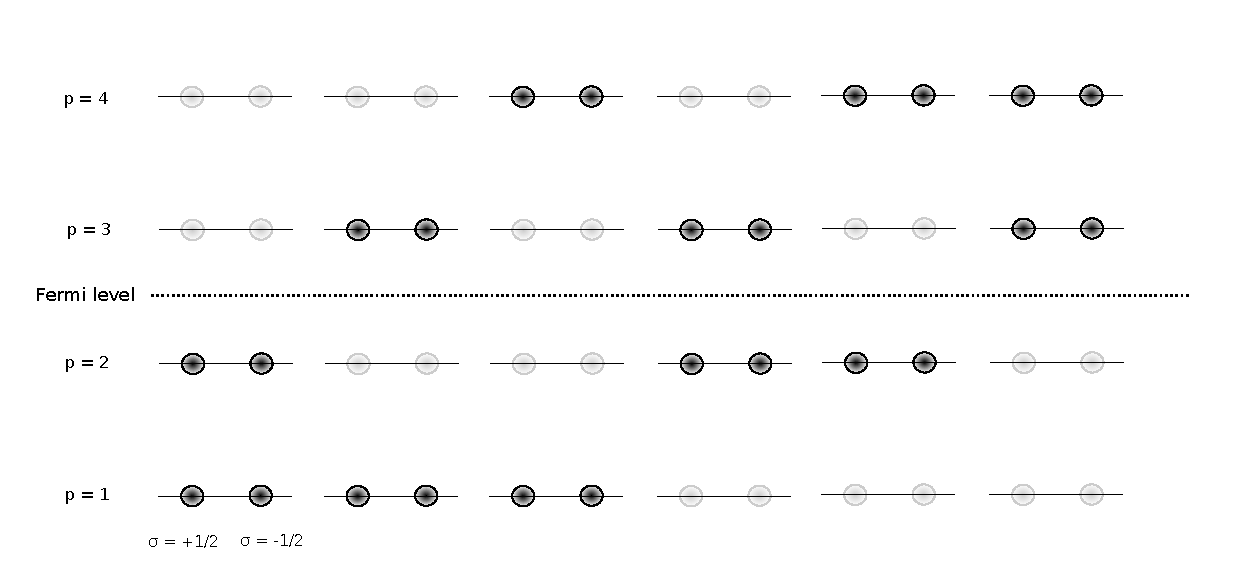
\includegraphics[width=1.1\linewidth]{Figures/Pairing_model2.pdf}
			\label{PairingModel_2}
			\caption{Configuration space for given pairing model showing all possible distributions of electrons}
		\end{figure}

 	We need to diagonalize the Hamiltonian matrix looking at the linear combination of all different compinations of 
	\begin{align}
		\hat{ \mathcal{H} } = \left(  \begin{matrix}
			& \left| \Phi_0 \right> & \left| \Phi_{12}^{56} \right> & \left| \Phi_{12}^{78} \right> & \left| \Phi_{34}^{56} \right> & \left| \Phi_{34}^{78} \right> & \left| \Phi_{1234}^{5678} \right> \\ 
			\left< \Phi_0 \right| &   &   &   &   &   & \\
			\left< \Phi_{12}^{56} \right| &   &   &   &   &   & \\
			\left< \Phi_{12}^{78} \right| &   &   &   &   &   & \\
			\left< \Phi_{34}^{56} \right| &   &   &   &   &   & \\
			\left< \Phi_{34}^{78} \right| &   &   &   &   &   & \\
			\left< \Phi_{1234}^{5678} \right| &   &   &   &   &   & 
		\end{matrix} \right)
	\end{align}

 Excluding the 4p-4h excitations one does not diagonalize the exact matrix, but rather the approximated matrix known from Configuration Interaction. 

 The diagonal elements are calculated using Wick's theorem. Looking first at the ground state calculation with the unperturbed Hamiltonian part
 \begin{align}
 	\left< \Phi_0 \middle| \hat{\mathbf{H_0}} \middle| \Phi_0 \right> 
 \end{align}
 \begin{align}
 	\left< \right|  a_{2 \downarrow}  a_{2 \uparrow} a_{1 \downarrow} a_{1 \uparrow} \sum_{p \sigma} \delta (p-1) a_{p \sigma}^{\dagger} a_{p \sigma} 
 	a_{1 \uparrow}^{\dagger} a_{1 \downarrow}^{\dagger} a_{2 \uparrow}^{\dagger} a_{2 \downarrow}^{\dagger} \left| \right> 
 \end{align}
 Which we see can contract in four different ways, resulting in 
 \begin{align}
 	2 \delta (1-1) + 2 \delta (2-1) = 2 \delta
 \end{align}

 And the perturbation part
 \begin{align}
 	\left< \Phi_0 \middle| \hat{\mathbf{V}} \middle| \Phi_0 \right>
 \end{align}
 \begin{align}
 	\left< \right| a_{2 \downarrow}  a_{2 \uparrow} a_{1 \downarrow} a_{1 \uparrow} \left( -g / 2 \sum_{pq} a_{p \uparrow}^{\dagger} a_{q \downarrow}^{\dagger} a_{q \downarrow} a_{p \uparrow} \right) 
 	a_{1 \uparrow}^{\dagger} a_{1 \downarrow}^{\dagger} a_{2 \uparrow}^{\dagger} a_{2 \downarrow}^{\dagger} \left| \right> 
 \end{align}
 As we can see, there are two ways this can contract, each contributing with the constant factor, $-g / 2$
 Resulting in the final Hamiltonian matrix 
 \begin{align}
 	\hat{\mathcal{H}} = \left( \begin{matrix}
 		2 \delta - g & -g / 2 & -g / 2 & -g / 2 & -g / 2 & 0  \\
 		-g / 2 & 4 \delta - g & -g / 2 & -g / 2 & 0 & -g / 2  \\
 		-g / 2 & -g / 2 & 6 \delta - g & 0 & -g / 2 & -g / 2 \\
 		-g / 2 & -g / 2 & 0 & 6 \delta - g & -g / 2 & -g / 2 \\
 		-g / 2 & 0 & -g / 2 & -g / 2 & 8 \delta - g & -g / 2 \\
 		0 & -g / 2 & -g / 2 & -g / 2 & -g / 2 & 10 \delta - g 
 	\end{matrix} \right)
 \end{align}

 \end{section}

 \begin{section}{Diagrammatic Rules}
 	One can visualize many-body quantum physics by using diagrams. 

 	
 \end{section}

 \begin{section}{Many-Body Perturbation Theory}
 	The Perturbation theory presents a non-iterative approach to approximating the ground state energy. The approach is similar to previous methods. We start by splitting the Hamiltonian into a solvable part and a perturbation. 
 	\begin{align}
 		\hat H = \hat H_0 + \hat V
 	\end{align}
 	Where we have chosen our basis such that
 	\begin{align}
 		\hat H_0 \left| \Psi_0 \right>  = W_0 \left| \Psi_0 \right>
 	\end{align}
 	We split the basis aswell
 	\begin{align}
 		\left| \Psi_0 \right> = \left| \Phi_0 \right> + \sum_i^{\infty} c_i \left| \phi_i \right>
 	\end{align}
 	Assuming intermediate normalization
 	\begin{align}
 		\left< \Phi_0 | \Psi_0 \right> = 1
 	\end{align}
	We can calculate the total exact energy
 	\begin{align}
 		E = \left< \Phi_0 \right| \hat H_0 \left| \Psi_0 \right> + \left< \Phi_0 \right| \hat V \left| \Psi_0 \right>
 	\end{align}
 	Where we know that
 	\begin{align}
 		 \left< \Phi_0 \right| \hat H_0 \left| \Psi_0 \right>  = W_0
 	\end{align}
 	And we get the corrolation energy
 	\begin{align}
 		E - W_0 = \Delta E = \left< \Phi_0 \right| \hat V \left| \Psi_0 \right>
 	\end{align}
 	We will usually aim to compute this energy when doing MBPT. 

 	\begin{subsection}{General derivation of Many Body Particle Theory equations}
 		Looking at the equation
 		\begin{align}
 			\hat V \left| \Psi_0 \right> = \hat H \left| \Psi_0 \right> + \hat H_0 \left| \Psi_0 \right> 
 		\end{align}
 		We reorganize and add the term $\omega \left| \Psi_0 \right>$ on both sides
 		\begin{align}
 			\hat V \left| \Psi_0 \right> + \omega \left| \Psi_0 \right> - \hat H \left| \Psi_0 \right> = \omega \left| \Psi_0 \right> - \hat H_0 \left| \Psi_0 \right> 
 		\end{align}
 		Remembering that $\hat H \left| \Psi_0 \right> = E\left| \Psi_0 \right> $, we get 
 		\begin{align}
 			\left| \Psi_0 \right> = \frac{ \hat V + \omega - E }{\omega - \hat H_0} \left| \Psi_0 \right>
 			\label{pert_1}
 		\end{align}
 		Before continuing, we introduce the operators $\hat P$ and $\hat Q$, such that
 		\begin{align}
 			\left| \Psi_0 \right> = \hat P \left| \Psi_0 \right> + \hat Q \left| \Psi_0 \right> 
 			&= \left| \Phi_0 \right> \left< \Phi_0 \middle| \Psi_0 \right> + \sum_i \left| \Phi_i \right> \left< \Phi_i \middle| \Psi_0 \right> 
 			\label{pert_2} \\
 			&= \left| \Phi_0 \right> + \chi
 		\end{align}
 		Giving
 		\begin{align}
 			\left| \Phi_0 \right> = \hat P \left| \Psi_0 \right> \;\;\;\; \chi = \hat Q \left| \Psi_0 \right> 
 			\label{pert_3}
 		\end{align}
 		Using $\hat R(\omega) = \frac{\hat{Q}}{\left( \omega - \hat H_0 \right)}$ and multiplying both sides with $\hat Q$ from the left in equation (\ref{pert_1}) we attain
 		\begin{align}
 			\hat Q \left| \Psi_0 \right> = \hat R(\omega) \left( \hat V + \omega - E \right) \left| \Psi_0 \right>
 		\end{align}
 		Using equations (\ref{pert_2}) and (\ref{pert_3}), we get
 		\begin{align}
 			\left| \Psi_0 \right> = \left| \Phi_0 \right> + \hat R(\omega) \left( \hat V + \omega - E \right) \left| \Psi_0 \right>
 		\end{align}
 		This is an iterative scheme. We can substitute $\left| \Psi_0 \right>$ on the right hand side with the entire right hand side. This results in an infinite sum provided the series converges
 		\begin{align}
 			\left| \Psi_0 \right> = \sum_0^\infty \left\{ \hat R(\omega) (\hat V + \omega - E) \right\}^m \left| \Phi_0 \right>
 		\end{align}
 		The right hand side does include the energy, $E$, which must be computed using $ E = W_0 + \Delta E$, and
 		\begin{align}
 			\Delta E = \left< \Phi_0 \right| \hat V \left| \Psi_0 \right> 
 			= \sum_0^\infty \left< \Phi_0 \right| \hat V \left[ \hat R(\omega) (\hat V - E + \omega) \right]^m \left| \Phi_0 \right>  
 		\end{align}
 	\end{subsection}

 	\begin{subsection}{Equations for Reileigh-Schrodinger Perturbation Theory}
 		We can interpret $\omega$ different ways. I here present the Reileigh-Schrodinger Perturbation Theory which postulates that
 		\begin{align}
 			\omega = W_0 
 		\end{align}
 		Such that 
 		\begin{align}
 			\left| \Psi_0 \right> = \frac{ \hat V - \Delta E }{\omega - \hat H_0} \left| \Psi_0 \right>
 		\end{align}
 		and we get the final equations
 		\begin{align}
 			\left| \Psi_0 \right> = \sum_0^\infty \left\{ \hat R(\omega) (\hat V + - \Delta E) \right\}^m \left| \Phi_0 \right>
 		\end{align}
 		and
 		\begin{align}
 			\Delta E = \sum_0^\infty \left< \Phi_0 \right| \hat V \left[ \hat R(\omega) (\hat V - \Delta E) \right]^m \left| \Phi_0 \right>  
 		\end{align}
 		Taking a closer look at the energy-equations, we find that we can write the first orders as
 		\begin{align*}
 			E^{(1)} &= \left< \Phi_0 \right| \hat V \left| \Phi_0 \right>  = V_{00}\\
 			E^{(2)} &= \left< \Phi_0 \right| \hat V \hat R_0 \hat V \left| \Phi_0 \right> \\
 			E^{(3)} &= \left< \Phi_0 \right| \hat V \hat R_0 (\hat V - E^{(1)})  \hat R_0 \hat V \left| \Phi_0 \right> \\
 			E^{(4)} &= \left< \Phi_0 \right| \hat V \hat R_0 (\hat V - E^{(1)})  \hat R_0 (\hat V - E^{(1)}) \hat R_0 \hat V \left| \Phi_0 \right> 
 					- E^{(2)} \left< \Phi_0 \right| \hat V \hat R_0^2 \hat V \left| \Phi_0 \right>\\
  		\end{align*}
  		Because of the frequent appearance, we can rewrite $\hat V - E^{(1)}$ as
  		\begin{align}
  			\hat \Omega = \hat V - E^{(1)}
  		\end{align}
  		We name this new variable the wave operator
 	\end{subsection}

 	\begin{subsection}{Canonical Hartree-Fock}
 		In the pairing model, we work with the Normal-ordered Hamiltonian
 		\begin{align}
 			\hat H_N = \hat F_N^d + \hat F_N^0 + \hat W		
 		\end{align}
 		Which is part of the total Hamiltonian by
 		\begin{align}
 			\hat H = \hat H_N + E_{\text{ref}}
 		\end{align}
 		Where
 		\begin{align}
 			\hat H_N \left| \Psi \right> = \Delta E \left| \Psi \right> 
 		\end{align}
 		If we use a Canonical Hartree-Fock basis, the Fock matrix will be diagonal, meaning 
 		\begin{align}
 			\hat F_N^o = 0 \;\;\; \text{     and  } \:\;\: f_{pq} = \epsilon_p \delta_{pq}
 		\end{align}
 		A noncanonical Hartree-Fock will be block diagonal with 
 		\begin{align}
 			f_{ia} = \left< i \right| \hat f \left| a \right> = 0
 		\end{align}

 	\end{subsection}

 	\begin{subsection}{Hartree-Fock calculations}
 		When doing Hartree-Fock calculation, we do a change of basis and instead of expanding our Hamiltonian, we vary the wavefunction to minimize the energy. We name the original basis by greek letters and the new basis by latin letters. The original basis should be chosen such that we can calculate the its expectation value. 
 		\begin{align}
 			\left< \Phi_0 \right| \hat H \left| \Phi_0 \right> = E^{\text{HF}}
 		\end{align}
 		Variational principle ensures that 
 		\begin{align}
 			E^{\text{HF}} > 0 
 		\end{align}
 		We now introduce a change of basis 
 		\begin{align}
 			\left| \psi_a \right> = \sum_{\lambda} C_{a\lambda} \left| \psi_{\lambda} \right>
 		\end{align}
 		Varying $C_{p\lambda}$, we can look for the basis providing the lowest energy. We start by rewriting $E^{HF}$ as a functional
 		\begin{align}
 			E\left[ \psi \right] = \sum_{a=1}^N \left< a \right| h \left| a \right> + \frac{1}{2} \sum_{ab}^N \left< ab \right| v \left| ab \right>
  		\end{align}
  		In terms of the original greek basis
  		\begin{align}
  			E\left[ \psi \right] = \sum_{a=1}^N \sum_{\alpha \beta} C_{a \alpha}^* C_{a \beta} \left< \alpha \right| h \left| \beta \right> + \frac{1}{2} \sum_{ab}^N \sum_{\alpha \beta \gamma \delta} C_{a \alpha}^* C_{b \beta}^* C_{a \gamma} C_{b \delta} \left< \alpha \beta \right| v \left| \gamma \delta \right>
  		\end{align}
  		To find the minima, we introduce a Lagrange multiplier before differentiating with respect to $C_{a  \alpha}^*$. This will give N equations, one for each state, $a$. The equations are given by
  		\begin{align}
  			\sum_{\beta} C_{a \beta} \left< \alpha \right| h \left| \beta \right> + \sum_b^N \sum_{\beta \gamma \delta} C_{b \beta}^* C_{b \delta} C_{a \gamma} \left< \alpha \beta \right| v \left| \gamma \delta \right> = \epsilon_a C_{a \alpha}
  		\end{align}
  		Defining
  		\begin{align}
  			h_{\alpha \gamma}^{\text{HF}} = \left< \alpha \right| h \left| \gamma \right> + \sum_{b=1}^N \sum_{\beta \delta} C_{b \beta}^* C_{b \delta} \left< \alpha \beta \right| v \left| \gamma \delta \right> 
  		\end{align}
  		We get the short hand iterative equations to be solved 
  		\begin{align}
  			\sum_{\gamma} h_{\alpha \gamma}^{\text{HF}} C_{a \gamma} = \epsilon_{a} C_{a \alpha}
  		\end{align}
 	\end{subsection}

 	\begin{subsection}{RSPT to for Pairing model}
 		
 		Given that our Hartree-Fock basis is canonical, $\hat F_N^0 = 0$, and $f_{pq} = \epsilon_p \delta_{pq}$, we can
  	\end{subsection}


 \end{section}

\end{chapter}




\begin{chapter}{Infinite Matter}
	A study of infinite matter is the most comprehensible way of studying nuclear material. This thesis will study the infinite electron gas before the final study of nuclear material. This is done because of pedagogical reasons and because the electron gas has closed form solutions that provide important benchmarking for the code. 
	\begin{section}{The Infinate Electron Gas}
		The infinite electron gas gives a good approximation to valence electrons in metal. The gas consist only of interacting electrons with a uniform background of charged ions. The whole system is charge neutral. We assume a cubic box, length $L$ and volume $\Omega = L^3$, with $N_e$ as the number of electrons with a charge density $\rho = N_e / \Omega$.

		We regard the system as homogenic, using the free particle normalized wave function
		\begin{align}
		 	\psi_{\vec k \sigma} (\vec r) = \frac{1}{\sqrt{\Omega}} e^{i \vec k \vec r} \xi_{\sigma}
		 \end{align}
		 Where $\vec k$ is the wave number and $\xi_{\sigma}$ is a spin function. 
		 \begin{align}
		 	\xi_{+\frac{1}{2}} = \left( \begin{matrix} 1 \\ 0 \end{matrix} \right) \:\;\:\; \xi_{-\frac{1}{2}} = \left( \begin{matrix} 0 \\ 1 \end{matrix} \right)
		 \end{align}
		 Assuming periodic boundary conditions, we acquire the following wave numbers
		 \begin{align}
		 	k_i = \frac{2\pi n_i}{L} \:\:\:\;\; i = x,y,z \;\;\:\:\: n_i = 0, \pm 1, \pm 2, ...
		 \end{align}
		 The electrons interact with the sentral symmetric Colomb potential, $\hat V(\vec r_1, \vec r_2)$ depending only on the distance $\left| \vec r_1 - \vec r_2 \right|$. 

		 The Hamiltonian for infinite electron gas is
		 \begin{align}
		 	\hat H = \hat T + \hat V
		 \end{align}
		 Where we have the kinetic energy, $\hat T$ as
		 \begin{align}
		 	\hat T = \sum_p \frac{\hbar ^2 k^2}{2m} a_{k \sigma}^{\dagger} a_{k \sigma}
		 \end{align}

	\end{section}
	\begin{section}{Infinite Nuclear Matter}
		Central to my thesis, is the study of infinite nuclear matter. I look at baryonic matter similar to the dense baryonic matter found in neutron stars. I limit the study to temperatures far below Fermi level. The matter is mostly made up of an equilibrium of baryons and leptons. In neutron star matter, we assume the equilibrium consist of protons, neutrons, electrons and muons with densities larger than $0.1 \text{fm}^-3$. The equilibrium conditions are specified by weak interactions
		\begin{align}
		 	b_1 \rightarrow b_2 + l + \bar \nu_l \:\:\:\:\:\: b_2 + l \rightarrow b_1 + \nu_l
		\end{align} 
		Where $b$ represent either neutron or proton and $l$ is either an electron or muon. $\nu_l$ is the corresponding neutrino. 

		Nuclear matter is a hypothetical system filling all of space at a uniform density. Symmetric nuclear matter (SNM) consist of equal numbers of protons of neutrons, while pure nuclear matter (PNM) consist only of neutrons. For finite-nucleus systems, the most difficult part is calculating the single particle wave function. For nuclear matter we can use plane wave basis and similar to electron gas, the difficult part is calculating the energy and the effective interaction between particles \cite{Day1967}. In my calculations, I have looked at pure nuclear matter. 


	\end{section}
	\begin{section}{Nuclear Interaction}
		Nuclear matter is composed of baryons, which interacts through the strong force. 
		
		\begin{subsection}{The Minnesota Potential}
			The Minnesota Potential is given as
			\begin{align}
				v(r) = &\left(v_R + (1 + P_{12}^\sigma) v_T/2 + (1 - P_{12}^\sigma) v_S/2 \right) \\
					   \cdot &\left( \alpha + (2- \alpha)P_{12}^r \right)/2 + (1+m_{t,1})(1+m_{t,2})\frac{e^2}{4r}
			\end{align}
			where $r$ is given as $\left| \mathbf{r_1} - \mathbf{r_2} \right|$ and $m_t$ is the isospin projection of particle 1 or 2. $m_t = \pm 1$. 
			$P_{12}^\sigma $ and $P_{12}^r$ are exchange operators for spin and position, respectively \cite{Baardsen}. Furthermore, we have used
			\begin{align} 
				v_R = v_{0R}e^{-k_R r^2}, \:\:\: v_T = -v_{0T} e^{-k_Tr^2}, \:\:\: v_S = -v_{0S}e^{-k_sr^2}
			\end{align}
			Where the constants $v_{0R}$, $v_{0T}$, $v_{0S}$, $k_R$, $k_T$ and $k_S$ are given by \cite{Thompson1977}
			\begin{enumerate}
				\item $v_{0R} = 200$MeV,  $k_R = 0.1487 \text{fm}^{-2}$
				\item $v_{0T} = 178$MeV,  $k_T = 0.649 \text{fm}^{-2}$
				\item $v_{0S} = 91.85$MeV, $k_S = 0.465 \text{fm}^{-2}$
			\end{enumerate}
			Written by second quantisation, we want to calculate the two-body interaction
			\begin{align}
			 	\left<k_p k_q \middle| v \middle| k_r k_s \right> = \frac{V_0}{L^3} \left(\frac{\pi}{\alpha}\right)^{3/2} e^{-q^2 / 4 \alpha} \delta_{\vec k_p + \vec k_q, \vec k_r + \vec k_s}
			\end{align}
			Where $q$ is the relative momentum transfer
			\begin{align}
				\mathbf{q} = \mathbf{p} - \mathbf{p'} 
			\end{align}
			\begin{align}
				\mathbf{p} = \frac{1}{2} (\mathbf{k}_p - \mathbf{k}_q) \:\:\:\:\: \mathbf{p'} = \frac{1}{2}(\mathbf{k}_r- \mathbf{k}_s) 
			\end{align}
			We can now set up the two-body Matrix-elements for the Minnesota Potential
			\begin{align}
				\left<\mathbf{k}_p \mathbf{k}_q \middle| v \middle| \mathbf{k}_r \mathbf{k}_s \right> = 
				&\left<\mathbf{k}_p \mathbf{k}_q \right| \frac{1}{2} \left( V_R + \frac{1}{2} V_T + \frac{1}{2} V_S \right) \left| \mathbf{k}_r \mathbf{k}_s \right>  \\
				+&\left<\mathbf{k}_p \mathbf{k}_q \right| \frac{1}{4} (V_T - V_S) P_{12}^\sigma \left| \mathbf{k}_r \mathbf{k}_s \right> \\
				-&\left<\mathbf{k}_p \mathbf{k}_q \right| \frac{1}{2} \left( V_R + \frac{1}{2} V_T + \frac{1}{2} V_S \right) P_{12}^\sigma P_{12}^\tau \left| \mathbf{k}_r \mathbf{k}_s \right> \\
				-&\left<\mathbf{k}_p \mathbf{k}_q \right| \frac{1}{4}(V_T - V_S) P_{12}^\tau  \left| \mathbf{k}_r \mathbf{k}_s \right>&
			\end{align}
			Matrix elements for the spin and isospin exchange operators are 
			\begin{align}
				\left< \sigma_p \sigma_q \right| P_{12}^\sigma \left| \sigma_r \sigma_s \right> = \delta_{\sigma_p,\sigma_s} \delta_{\sigma_q,\sigma_r}
			\end{align}
			One can see that these matrix elements come at a far greater computational cost than for electron-electron interaction in the electron gas. Therefore it is necessary to compute and store all elements instead of computing them "on the fly". Source: Lecture 1-2 infinite matter. 
		\end{subsection}
		
	\end{section}
\end{chapter}




\begin{chapter}{Implementation}
	In this thesis I have created three different solvers for Coupled Cluster Doubles equations. 
	\begin{enumerate}
		\item A naive brute force implementation of the equations summing over all variables. 
		\item A naive brute force implementation of intermediate equations summing over all variables.
		\item Rewriting summations as matrix-matrix multiplications and exploiting various symmetry arguments one can set up a block implementation.
	\end{enumerate}	
	There is a significant performance leap between each method, but I have included the first two solvers for both educational and benchmarking purposes. The Pairing model with 4 particles and 4 holes is a small system that one can easily solve using the naive approach. After producing expected results with the naive solver, I have compared the more complicated solvers to the naive solver for all systems. 

	\begin{section}{Implementing the CCD equations}
		The basic steps of all implemented CCD algorithms can be explained through these steps
		\begin{enumerate}
			\item Initialize amplitudes $t^{(0)} = 0$ and $\Delta E_{CCD}^{(0)} = 0$
			\item Update the amplitudes and calculate $\Delta E_{CCD}^{(1)}$
			\item If $ |\Delta E_{CCD}^{(1)} - \Delta E_{CCD}^{(0)}| \geq \epsilon $, update amplitudes and compute $\Delta E_{CCD}^{2}$
			\item Repeat until $ |\Delta E_{CCD}^{(n+1)} - \Delta E_{CCD}^{(n)}| \leq \epsilon $
		\end{enumerate}
		The difference between the three solvers I have implemented is the way I update amplitudes. The naive brute force solver loops over all indices when computing. An example of diagram $L_a$ is shown below

		\begin{lstlisting}
		for i in 0, ..., Nholes:
			for j in 0, ..., Nholes:
				for a in Nholes, ..., Nparticles:
					for b in Nholes, ..., Nparticles:
						for c in Nholes, ..., Nparticles:
							for d in Nholes, ..., Nparticles:
								tnew(a,b,i,j) = 0.5  v(a,b,c,d)  told(c,d,i,j)
		\end{lstlisting}

		A significant cost reduction can be obtained by factorizing the diagrams as shown in equation (\ref{Intermediates}). By calculating the four intermediate diagrams, $I_1$, $I_2$, $I_3$ and $I_4$ beforehand and storing the results reduce the cost of calculation from $\mathcal{O}(h^4 p^4)$ to $\mathcal{O}(h^4 p^2)$. The second solver applies this method. 

	\end{section}

	\begin{section}{Matrix Representation of Contractions}
		Diagrams can be viewed as contractions of tensors of varying degree. An example is the matrix-matrix multiplication product
		\begin{align}
		 	\left( M N \right)_{\gamma}^{\alpha} = \sum_{\beta} M_{\beta}^\alpha N_\gamma^\beta 
		 	\label{matrix matrix multiplication}
		\end{align} 

		As our goal is to rewrite the Coupled Cluster equations as matrix-matrix products. We will need to map tensors of rank $\geq 2$ onto matrices. One mapping that provides systematic and unique matrix elements can be 
		\begin{align}
			\left<pq\middle| \hat v\middle|rs\right> = V_{\alpha(p,q),\beta(r,s)}
		\end{align}
		Where 
		\begin{align}
			\alpha(p,q) = p + q N_p \;\,\:\; \beta(r,s) = r + s N_r
			\label{mapping of matrix elements}
		\end{align}
		We need to be careful when mapping tensors this way. Consider first the calculation of the perfectly aligned $L_a$ term
		\begin{align}
			L_a = \sum_{cd} \left< ab \middle| \hat v\middle|cd\right> t_{ij}^{cd}
		\end{align}
		Mapping this equation using equation (\ref{mapping of matrix elements})
		\begin{align}
			\left< ab \middle| \hat v\middle|cd\right> = v_{ab}^{cd} \rightarrow V_{\beta(c,d)}^{\alpha(a,b)}
		\end{align}
		and
		\begin{align}
			t_{ij}^{cd} \rightarrow T_{\delta(i,j)}^{\beta(c,d)}
		\end{align}
		As we are mapping to unique elements 
		\begin{align}
			\beta(c,d) = \beta(c,d)
		\end{align}
		We can now rewrite the equation 
		\begin{align}
			(L_a)_ \delta^\alpha = \sum_ \beta V_ \beta^\alpha T_ \delta^\beta
		\end{align}
		Implying by regarding equation (\ref{matrix matrix multiplication}) that we can rewrite the product as matrix-matrix multiplication 
		\begin{align}
			L_a = VT
		\end{align}

		\begin{subsection}{Aligning elements}	
			Unfortunately, not all product are perfectly aligned like $L_a$. Consider, for example, the term, $L_c$
			\begin{align}
				L_c = -P\left(ij\middle|ab\right) \sum_{kc} \left<kb\middle|\hat v\middle|cj\right>t_{ik}^{ac}
			\end{align}
			Using the same mapping scheme
			\begin{align}
				\left<kb\middle|\hat v\middle|cj\right> = v_{cj}^{kb} \rightarrow V_{\beta(cj)}^{\alpha(kb)}
			\end{align}
			and
			\begin{align}
				t_{ik}^{ac} \rightarrow T_{\delta(ik)}^{\gamma(ac)}
			\end{align}
			This matrix multiplication is misaligned, and if the number of particles is unequal to the number of holes, the matrices' size will uncompatible. 
			\begin{align}
				(L_c)_ \delta^\alpha \neq -P\left(ij\middle|ab\right) \sum_ \beta V_{\beta(cj)}^{\alpha(kb)} T_{\delta(ik)}^{\gamma(ac)}
			\end{align}
			We need to find another mapping, such that
			\begin{align}
				v_{cj}^{kb} \rightarrow \tilde V_{\beta(ck)}^{\alpha(bj)}
			\end{align}
			and 
			\begin{align}
				t_{ik}^{ac} \rightarrow \tilde T_{\delta(ia)}^{\gamma(ck)}
			\end{align}
			Now, the matrix multiplication is aligned
			\begin{align}
				(\tilde L_c)_ \delta^\alpha = -P\left(ij\middle|ab\right) \sum_ \beta \tilde V_{\beta(ck)}^{\alpha(bj)} \tilde T_{\delta(ia)}^{\gamma(ck)}
			\end{align}
			Note, however, that 
			\begin{align}
				L_c \neq \tilde L_c
			\end{align}
			We must "realign" $\tilde L_c$ to match the correct diagram
			\begin{align}
				(\tilde L_c)_{\delta(i,a)}^{\alpha(b,j)} \rightarrow (L_c)_{\delta(i,k)}^{\alpha(k,b)}
			\end{align}

			Another example is the $Qc$ term
			\begin{align}
				Q_c = -\frac{1}{2} \hat P(ij) \sum_{klcd} \left< kl \middle| v \middle| cd \right> t_{ik}^{ab} t_{jl}^{cd} 
			\end{align}
			We can rewrite this as a matrix-matrix multiplication with the matrix elements given by
			\begin{align}
				\left< kl \middle| v \middle| cd \right> = v_{cd}^{kl} & \rightarrow V^{\alpha(cd)}_{\beta(kl)} \\
				t_{ik}^{ab} & \rightarrow (T_1)_{\gamma(ik)}^{\delta(ab)} \\
				t_{jl}^{cd} & \rightarrow (T_2)_{\omega(jl)}^{\eta(cd)}
			\end{align}
			Because we sum over the coefficients $klcd$, we must make sure that they belong to the "inner" indexes. This can only be done by creating a hole, particle-particle-hole configuration. We must also change the order of multiplication
			\begin{align}
				V^{\alpha(cd)}_{\beta(kl)} &  \rightarrow \tilde V^{\delta(k)}_{\gamma(cdl)} \\
				(T_1)_{\gamma(ik)}^{\delta(ab)} & \rightarrow \tilde (T_1)^{\alpha(abi)}_{\delta(k)} \\
				(T_2)_{\omega(jl)}^{\eta(cd)} & \rightarrow \tilde (T_2)^{\gamma(cdl)}_{\beta(j)}
			\end{align}
			This gives us
			\begin{align}
				( \tilde Q_c )_{\beta(j)}^{\alpha(abi)} = -\frac{1}{2} \hat P(ij) \sum_{klcd} (\tilde T_1)^{\alpha(abi)}_{\delta(k)} \tilde V^{\delta(k)}_{\gamma(cdl)} (\tilde T_2)^{\gamma(cdl)}_{\beta(j)}
			\end{align}
			Which must be realigned back to the properly aligned $Q_c$ before it can be added to the amplitude equations.
			\begin{align}
				( \tilde Q_c )_{\beta(j)}^{\alpha(abi)} \rightarrow (Q_c)_{\beta(ij)}^{\alpha(ab)}
			\end{align}
			We will need a general mapping function that can be used regardless of the amount of states used. It turns out that we can use the same mapping as before, just generalized to $N$ states.
			\begin{align}
				\alpha(p_1,p_2,p_3,...,p_N) = p_1 + p_2N_1 + p_3N_1N_2 + ... + p_N N_1 N_2 ... N_{N-1} 
			\end{align}
			Where $N_n$ determines the maximum number of states for $p_n$. If for example $p_n \in i$, i.e. $p_n$ is a hole-state, $N_n = N_{holes}$.

			Writing the diagrams as matrix-matrix multiplications serves as a significant reduction of computational time, due to the efficient algortithms in the BLAS-packages for matrix-matrix multiplications. However, since one has to save all the matrices, memory usage will be a problem for large basises. 
		\end{subsection}

	\end{section}

	\begin{section}{Block Implementation}
		One can both greatly reducing memory usage and improve computational speed by exploiting symmetries for infinite matter . Due to kroenecker delta's in the interaction, one such symmetry is the conservation of momentum
		\begin{align}
			\delta_{\vec k_p + \vec k_q, \vec k_r + \vec k_s} \rightarrow \vec k_p + \vec k_q = \vec k_r + \vec k_s
		\end{align}
		We also conserve spin 
		\begin{align}
			m_{s_p} + m_{s_q} = m_{s_r} + m_{s_s}
		\end{align}
		and for nuclear matter, we will conserve isospin aswell
		\begin{align}
			m_{t_p} + m_{t_q} = m_{t_r} + m_{t_s}
		\end{align}
		The amplitudes will be subject to the same restrictions, vizualised by the first order amplitude generated by perturbation theory
		\begin{align}
			(t_{ij}^{ab})^{t=0} = \frac{\left<ab\middle|\hat v\middle|ij\right>}{\epsilon_i + \epsilon_j - \epsilon_a - \epsilon_b}
		\end{align}
		Looking at the $L_a$ term
		\begin{align}
			L_a = \sum_{cd} \left<ab\middle|\hat v\middle|cd\right> t_{ij}^{ab}
		\end{align}
		We see that 
		\begin{align}
			\vec k_a + \vec k_b = \vec k_c + \vec k_d = \vec k_i + \vec k_j
		\end{align}
		And the same for spin
		\begin{align}
			m_{s_a} + m_{s_b} = m_{s_c} + m_{s_d} = m_{s_i} + m_{s_j} 
		\end{align}
		When summing over all variations of contractions, only the quantum numbers preserving the symmetry requirements are nonzero. When storing the interactions in a matrix, most of it will have zero-elements. The blocking method will store the nonzero parts in blocks inside the matrix. By keeping track of the blocks, we can reduce the full matrix-matrix multiplication to a series of multiplications of the blocks. We will hereby refer to the series of blocks as \textit{channels}.

		\begin{subsection}{Two-state configurations}
			As we can see from the $L_a$ diagram, the conservation laws apply for a combination of two states. The next step is then to set up all two-state configurations that will be needed. We start by setting up the direct two-state channels, $T$, which consist of all two-hole and two-particle configurations. A unique identifier must be set up for the combination of quantum numbers. The identifier is used to aligning the non-zero combinations of two-body states to the same channel. Without this identifier, we will have to loop over all channels for each two-body state. I have used the following function 
			\begin{align}
				\text{Index}(N_x,N_y,N_z,S_z,T_z) = &2(N_x + m)M^3 + 2(N_y+m)M^2 + \\ & 2(N_z+m)M + 2(S_z+1) + (T_z+1)
			\end{align}
			Using the same logic as in equation (\ref{mapping of matrix elements}) to get a unique identifier for every combination of $N_x,N_y,N_z,S_z$ and $T_z$. Which imply that the two-body states have the same momentum, spin and isospin projection, which satisfies our conservation laws. We need $m$ and $M$ to be sufficiently large. I have used
			\begin{align}
				m = 2|\sqrt{N_{\text{max}}}| \:\:\:\:\:\: M = 2m +1
			\end{align}
			Because of the Pauli-exclusion, two particles cannot occupy the same state, so we can further reduce the amount of two-body states by excluding equal one-body states from the channels. An algorithm for setting up the direct channels can be portraied as
			\begin{align*}
				&\mathbf{for } \text{ one-body state 1} \in \text{STATES}: \\
				&\:\:\:\: \mathbf{for } \text{ one-body state 2} \in \text{STATES}: \\
				&\:\:\:\:\:\:\:\: \mathbf{if} \text{ one-body state 1} \neq \text{ one-body state 2}: \\
				&\:\:\:\:\:\:\:\:\:\: N_x = n_{x,1} + n_{x,2} \\
				&\:\:\:\:\:\:\:\:\:\: N_y = n_{y,1} + n_{y,2} \\
				&\:\:\:\:\:\:\:\:\:\: N_z = n_{z,1} + n_{z,2} \\
 				&\:\:\:\:\:\:\:\:\:\: S_z = m_{s,1} + m_{s,2} \\
				&\:\:\:\:\:\:\:\:\:\: T_z = m_{t,1} + m_{t,2} \\
				&\:\:\:\:\:\:\:\:\:\: \text{Id} = \text{Index}(N_x,N_y,N_z,S_z,T_z) \\
				&\:\:\:\:\:\:\:\:\:\: T \leftarrow (\text{ one-body state 1}, \text{ one-body state 2}, \text{ Id})
			\end{align*}

		\end{subsection}
		
		\begin{subsection}{Unaligned channels}
			Diagram $L_a$, $L_b$ and $Q_a$ have conservation requirements as shown previously for $L_a$
			\begin{align}
			 	\mathbf{k}_a + \mathbf{k}_b = \mathbf{k}_c + \mathbf{k}_d = \mathbf{k}_i + \mathbf{k}_j 
			\end{align}
			Which are implemented using the direct channels. We will however run into some trouble when computing the unaligned diagrams $L_c$, $Q_b$, $Q_c$ and $Q_d$. The $L_c$ diagram is given by 
			\begin{align}
				L_c = - \hat P(ij|ab) \sum_{kc} \left<kb\middle|\hat v\middle| cj \right> t_{ik}^{ac}
			\end{align}
			Looking at the conservation requirement for $L_c$
			\begin{align}
				\mathbf{k}_k + \mathbf{k}_b = \mathbf{k}_c + \mathbf{k}_j = \mathbf{k}_a + \mathbf{k}_c = \mathbf{k}_i + \mathbf{k}_k
			\end{align}
			and 
			\begin{align}
				m_{s,k} + m_{s,b} = m_{s,c} + m_{s,j}  \:\:\:\:\:\:\: m_{t,k} + m_{t,b} = m_{t,c} + m_{t,j} 
			\end{align}
			When realigning the equation, we want it to be
			\begin{align}
				\tilde Lc = -\hat P(ij|ab) \sum_{kc} \left<bj | \tilde v | ck \right> \left< ck \right| \tilde t \left| ai \right>
			\end{align}
			We reorganize the conservation requirements as well to make sure we only calculate the non-zero terms
			\begin{align}
				\mathbf{k}_b - \mathbf{k}_j = \mathbf{k}_c - \mathbf{k}_k = \mathbf{k}_c - \mathbf{k}_k = \mathbf{k}_i - \mathbf{k}_a
			\end{align}
			Spin and isospin will be subject to the same reorganizing. We see that the direct channels do not represent the right conservation requirement and we must set up the cross channels, $X$, that consist of particle-hole or hole-particle two-body configurations. An algorithm can be set up as
			\begin{align*}
				&\mathbf{for } \text{ one-body state 1} \in \text{STATES}:\\
				&\:\: \mathbf{for } \text{ one-body state 2} \in \text{STATES}:\\
				&\:\:\:\: \mathbf{if} \text{ one-body state 1} \neq \text{ one-body state 2}:\\
				&\:\:\:\:\:\: N_x = n_{x,1} - n_{x,2} \\
				&\:\:\:\:\:\: N_y = n_{y,1} - n_{y,2} \\
				&\:\:\:\:\:\: N_z = n_{z,1} - n_{z,2} \\
 				&\:\:\:\:\:\: S_z = m_{s,1} - m_{s,2} \\
				&\:\:\:\:\:\: T_z = m_{t,1} - m_{t,2} \\
				&\:\:\:\:\:\: \text{Id} = \text{Index}(N_x,N_y,N_z,S_z,T_z) \\
				&\:\:\:\:\:\: X \leftarrow (\text{ one-body state 1}, \text{ one-body state 2}, \text{ Id}) \\
				&\:\:\:\:\:\: \text{Id}' = \text{Index}(-N_x,-N_y,-N_z,-S_z,-T_z) \\
				&\:\:\:\:\:\: X' \leftarrow (\text{ one-body state 2}, \text{ one-body state 1}, \text{ Id'})
			\end{align*}
			Where $X'$ is the cross channel compliment, $X(pq) = X'(qp)$. The coss-channels are used for calculating $Q_b$ and $L_c$. 

			Looking at the diagram $Q_c$
			\begin{align}
				Q_c = -\frac{1}{2} \hat P(ij) \sum_{klcd} \left<kl|\hat v|cd\right> t_{ik}^{ab} t_{jl}^{cd}
			\end{align}
			With the momentum conservation requirement
			\begin{align}
				\mathbf{k}_k + \mathbf{k}_l = \mathbf{k}_c \mathbf{k}_d = \mathbf{k}_i + \mathbf{k}_k = \mathbf{k}_a + \mathbf{k}_b = \mathbf{k}_j + \mathbf{k}_l = \mathbf{k}_c + \mathbf{k}_d
			\end{align}
			We see that we must realign the diagram as
			\begin{align}
				\tilde Q_c = -\frac{1}{2} \hat P(ij) \sum_{klcd} \left<abi\right|\tilde t\left|k\right> \left<k\right|\tilde v\left|cdl\right> \left<cdl\right|\tilde t\left|j\right>
			\end{align}
			Which set the conservation requirement as 
			\begin{align}
				\mathbf{k}_a + \mathbf{k}_b	- \mathbf{k}_i = \mathbf{k}_k = \mathbf{k}_k = \mathbf{k}_c + \mathbf{k}_d - \mathbf{k}_l = \mathbf{k}_c + \mathbf{k}_d - \mathbf{k}_l = \mathbf{k}_j
			\end{align}
			We set up three-body and corresponding one-body channels to calculate $Q_c$ and $Q_d$. An example algorithm for the $K_h$ and $K_{p,p,h}$ channels can be outlined as
			\begin{align*}
				&\mathbf{for } \text{ one-body state 1 } \in \text{HOLES}:\\
				&\:\: N_x = n_{x,1}\\
				&\:\: N_y = n_{y,1}\\
				&\:\: N_z = n_{z,1}\\
 				&\:\: S_z = m_{s,1}\\
				&\:\: T_z = m_{t,1}\\
				&\:\: \text{Id} = \text{Index}(N_x,N_y,N_z,S_z,T_z) \\
				&\:\: K_h \leftarrow (\text{ one-body state 1}, \text{ Id}) \\ \\ \\ 
				&\mathbf{for } \text{ one-body state 1} \in \text{PARTICLES}: \\
				&\:\: \mathbf{for } \text{ one-body state 2} \in \text{PARTICLES}: \\
				&\:\:\:\: \mathbf{for } \text{ one-body state 3} \in \text{HOLES}: \\
				&\:\:\:\:\:\: \mathbf{if} \text{ one-body state 1} \neq \text{ one-body state 2}: \\
				&\:\:\:\:\:\:\:\: N_x = n_{x,1} + n_{x,2} - n_{x,3}\\
				&\:\:\:\:\:\:\:\: N_y = n_{y,1} + n_{y,2} - n_{y,3}\\
				&\:\:\:\:\:\:\:\: N_z = n_{z,1} + n_{z,2} - n_{z,3}\\
 				&\:\:\:\:\:\:\:\: S_z = m_{s,1} + m_{s,2} - n_{s,3}\\
				&\:\:\:\:\:\:\:\: T_z = m_{t,1} + m_{t,2} - n_{t,3}\\
				&\:\:\:\:\:\:\:\: \text{Id} = \text{Index}(N_x,N_y,N_z,S_z,T_z) \\
				&\:\:\:\:\:\:\:\: K_{p,p,h} \leftarrow (\text{ one-body state 1}, \text{ one-body state 2}, \text{ one-body state 3},  \text{ Id}) \\
			\end{align*}
		\end{subsection}

		\begin{subsection}{Permutations}
			Some diagrams come with permutations. These are easy to handle by simply interchanging indexes when adding the diagram to $t^{(n+1)}$. 
			\begin{align*}
				&\mathbf{for } \text{ i} \in \text{Holes}: \\
				&\:\:\mathbf{for } \text{ j} \in \text{Holes}: \\
				&\:\:\:\:\mathbf{for } \text{ a} \in \text{Particles}: \\
				&\:\:\:\:\:\:\mathbf{for } \text{ b} \in \text{Particles}: \\
				&\:\:\:\:\:\:\:\: t^{(n+1)}(a,b,i,j) = t^{(n+1)} - \frac{1}{2}\left(Q_c(a,b,i,j) - Q_c(a,b,j,i)\right)
			\end{align*}
		\end{subsection}

	\end{section}

	\begin{section}{Setting Up Basis}
		Before doing coupled cluster calculations, the basis must be set up. An important property of this basis, is the occupied and virtual states. For infinite nuclear matter, the following algorithm can be used to set up the states. This algorithm should reproduce the magic numbers presented. 
		\begin{align*}
			&\mathbf{for } \text{ shell } \in \text{ All Shells}: \\
			&\:\:\:\mathbf{for } \: n_x, n_y, n_z \in [-\text{shell, shell} ]: \\
			&\:\:\:\:\:\:n = n_x^2 + n_y^2 + n_z^2 \\
			&\:\:\:\:\:\:\mathbf{if }\: n = \text{shell}: \\
			&\:\:\:\:\:\:\:\:\:\mathbf{for } \: m_s \in \{-1,1\} \\
			&\:\:\:\:\:\:\:\:\:\:\:\: \mathbf{for } \: m_t \in \{-1,1\} \\
			&\:\:\:\:\:\:\:\:\:\:\:\:\:\:\:\text{States} \leftarrow (e, n_x, n_y, n_z, m_s, m_t) \\
			&\:\:\:\:\:\:\:\:\:\:\:\:\:\:\:N_s = N_s + 1 \\
			&\:\:\:\:\:\:\:\:\:\:\:\:\:\:\:\mathbf{if } \text{ shell} < \text{ Fermi level}: \\
			&\:\:\:\:\:\:\:\:\:\:\:\:\:\:\:\:\:\: N_h = N_h + 1
		\end{align*}
	\end{section}

	\begin{section}{Parallellization}
		An important part of optimizing the code, is by setting up a parallell code. By doing this, we can fully utilize the capacity of computers with many processing cores. I have, in this project, used the Super Computer Smaug located at Institute of Physics at the University of Oslo. 
	\end{section}

\end{chapter}




\begin{chapter}{Results}
	
	\begin{section}{The Pairing Model}
		The Pairing Model serve as a valuable benchmark for implemented solvers. As I have looked at a 4p4h configuration, a full configuration interaction solver can be implemented giving the exact solution. One can also calculate the exact solution for second order perturbation theory by hand \cite{Hjorth-Jensen2016}. 
		\begin{align}
			\Delta E_{MBPT2} = \frac{1}{4} \sum_{abij} \frac{\left<ij\middle|\middle|ab\right>\left<ab\middle|\middle|ij\right>}{\epsilon_{ij}^{ab}} = 
			\sum_{a<b,i<j} \frac{\left<ij\middle|\middle|ab\right>\left<ab\middle|\middle|ij\right>}{\epsilon_{ij}^{ab}}
		\end{align}
		Where 
		\begin{align}
			\epsilon_{ij}^{ab} = \epsilon_i + \epsilon_j - \epsilon_a - \epsilon_b
		\end{align}
		and
		\begin{align}
			\epsilon_p = h_{pp} + \sum_i \left<pi\middle|\middle|pi\right>
		\end{align}
		This results in
		\begin{align}
			\Delta E_{MBPT2} = \frac{\left<01\middle|\middle|45\right>^2}{\epsilon_{01}^{45} } + \frac{\left<01\middle|\middle|67\right>^2}{\epsilon_{01}^{67} }
							  +\frac{\left<23\middle|\middle|45\right>^2}{\epsilon_{23}^{45} } \ \frac{\left<23\middle|\middle|67\right>^2}{\epsilon_{23}^{67} }
		\end{align}
		\begin{align}
			\Delta E_{MBPT2} = -\frac{g^2}{4} \left( \frac{1}{4+g} + \frac{1}{6+g} + \frac{1}{2+g} + \frac{1}{4+g} \right)
		\end{align}
		Where g represents the interaction strength. The table below shows my results for various g's both using the exact mbpt2 calculations and my numerically computed results. All results can be accessed on github \cite{WholmenGithub}

		\begin{table}
			\begin{center}
				\begin{tabular}[center]{l | c | c | r}
					g & $E_0$ & exact $ \Delta E_{MBPT2}$  & $\Delta E_{MBPT2}$ \\
					\hline
					-1 & 3 & -0.466667 & -0.466667 \\
					-0.5 & 2.5 & -0.0887446 & -0.0887446 \\
					0 & 2 & 0 & 0 \\
					0.5 & 1.5 & -0.0623932 & -0.0623932 \\
					1 & 1 & -0.219048 & -0.219048
				\end{tabular}
			\end{center}
			\caption{A table showing corrolation energies for Pairing model with 4 particle-states and 4 hole-states.  }
			\label{Results1}
		\end{table}
		As one can see, the corrolation energies computed perfectly matches which both tells us that the basis set is set up correctly and that the MBPT2 solver is set up correctly. The results presented also match the results found in \cite{Hjorth-Jensen2016}

		The second order perturbation theory is valuble for benchmarking my implementation of Coupled Cluster Doubles. By initializing the first set of amplitudes, $t$, as zero, I get
		\begin{align}
			t_{ij}^{ab(0)} = 0  
		\end{align}
		\begin{align}
			t_{ij}^{ab(1)} = \frac{1}{4} \sum_{ijab} \frac{\left<ab\middle|\middle|ij\right>}{\epsilon_{ij}^{ab}} 
 		\end{align}
 		Which is equal to second order pertubation theory. 
 		\begin{table}
			\begin{center}
				\begin{tabular}[center]{l | c | r}
					g & $ \Delta E_{MBPT2}$  & $\Delta E_{CCD}^{(1)}$ \\
					\hline
					-1 & -0.466667 & -0.466667 \\
					-0.5 & -0.0887446 & -0.0887446 \\
					0 & 0 & 0 \\
					0.5 & -0.0623932 & -0.0623932 \\
					1 & -0.219048 & -0.219048
				\end{tabular}
			\end{center}
			\caption{A table comparing corrolation energies for Pairing model with 4 particle-states and 4 hole-states. This table show that CCD solver used with only a single iteration produces results exactly equal to mbpt2. This was done with the naive implementation of CCD equations}
			\label{Results2}
		\end{table}

		\begin{subsection}{Comparison of CCD solvers}
			In this thesis I have created three different solvers for Coupled Cluster Doubles equations. 
			\begin{enumerate}
				\item A naive brute force implementation of the equations summing over all variables. 
				\item A naive brute force implementation of intermediate equations summing over all variables.
				\item Rewriting summations as matrix-matrix multiplications and exploiting various symmetry arguments one can set up a block implementation.
			\end{enumerate}		
			As shown in table (\ref{Results2}), the naive implementation reproduces the mbpt2 energies as expected. I have used both the naive and intermediate CCD solver to compute corrolation energies for the Pairing model and again, \cite{Hjorth-Jensen2016} provides us with a good benchmark for the CCD equations.

			\begin{table}
				\begin{center}
					\begin{tabular}[center]{l | c | r}
						g & $ \Delta E_{CCD}$ Naive  & $\Delta E_{CCD}$ Intermediates \\
						\hline
						0 & x & x \\
						-0.5 & -0.0630564 & -0.0630562 \\
						0 & 0 & 0 \\
						0.5 & -0.0833621 & -0.0833623 \\
						1 & -0.369557 & -0.369557
					\end{tabular}
				\end{center}
				\caption{A table comparing corrolation energies for Pairing model with 4 particle-states and 4 hole-states. This table compare results from Naive and Intermediate implementation of CCD equations. A relaxing factor of $w = 0.3$ has been used because of divergence around $g=-1$}
				\label{Results3}
			\end{table}
			As one can see, my solvers reproduce results presented in \cite{Hjorth-Jensen2016}. For values of $g$ close to $-1$, one will see a divergence for CCD equations. By introducing a relaxing factor of $w = 0.3$, this problem was solved. 
  
		\end{subsection}
		\begin{subsection}{Comparison of various solvers}
			The full configuration interaction provides us with the exact solution for the 4p4h Pairing model. It can therefore be useful to compare the performance of Perturbation theory to second, third and fourth order with Coupled Cluster Doubles and configuration interaction without the four-particle excitation. 
			\begin{figure}H
				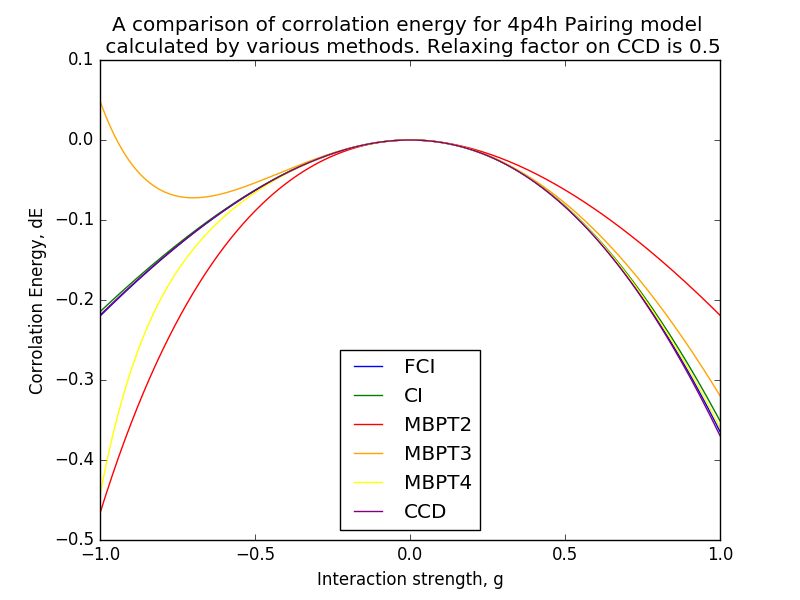
\includegraphics[width=\linewidth]{../Pairing_Model/Results/Figures/Pairing4p4h_CompareDE_AllMethods.png}
				\caption{Comparing }
				\label{Results4}
			\end{figure}

			\begin{figure}
				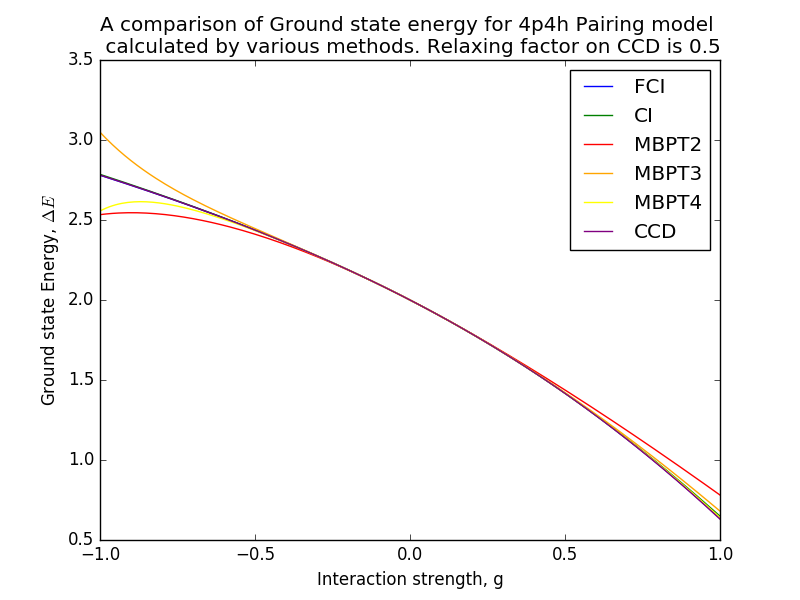
\includegraphics[width=\linewidth]{../Pairing_Model/Results/Figures/Pairing4p4h_CompareE_AllMethods.png}
				\caption{}
				\label{Results5}
			\end{figure}

		\end{subsection}


	\end{section}

\end{chapter}




\begin{chapter}{Appendix}
	
\end{chapter}

\medskip


\begin{thebibliography}{9}

	\bibitem{Baardsen}
	Gustav Baardsen
	\textit{Coupled-cluster theory for infinite matter} 2014

	\bibitem{ShavittAndBartlett}
	Isaiah Shavitt and Rodney J. Bartlett
	\textit{Many-Body Methods in Chemistry and Physics} 2009

	\bibitem{Szabo}
	Attila Szabo and Neil S. Ostlund
	\textit{Modern Quantum Chemistry. Introduction to Advanced Electronic Structure Theory} 1982

	\bibitem{Griffiths}
	David J. Griffiths
	\textit{Introduction to Quantum Mechanics} Second edition 2005

	\bibitem{Sakurai}
	J.J. Sakurai
	\textit{Modern Quantum Mechanics} Revised Edition 1993

	\bibitem{Hjorth-Jensen2016}
	Morten Hjorth-Jensen, Maria Paola Lombardo and Ubiraja van Kolck
	\textit{An Advanced Course in Computational Nuclear Physics} 2016

	\bibitem{Raimes}
	Stanley Raimes
	\textit{Many-Electron Theory} 1972

	\bibitem{Day1967} 
	B. D. Day
	\textit{Rev. Mod. Phys.,}
	39:719, 1967.

	\bibitem{Thompson1977}
	D. R. Thompson, M. Lemere and Y.C. Tang.
	\textit{Nucl. Phys. A,} 286:53 1977.

	\bibitem{WholmenGithub}
	Fredrik Wilhelm Holmen
	\textit{https://github.com/wholmen/Master} 

\end{thebibliography}


\end{document}